\title{Extrapolating expected accuracies for multi-class classification}
\author{Charles Zheng, Rakesh Achanta and Yuval Benjamini}
\date{\today}

\documentclass[12pt]{article} 

% packages with special commands
\usepackage{amssymb, amsmath}
\usepackage{epsfig}
\usepackage{array}
\usepackage{ifthen}
\usepackage{color}
\usepackage{fancyhdr}
\usepackage{graphicx}
\usepackage{mathtools}
\usepackage{csquotes}
\usepackage{multirow}
\usepackage{xcolor}

\newcommand\crule[3][black]{\textcolor{#1}{\rule{#2}{#3}}}


\definecolor{grey}{rgb}{0.5,0.5,0.5}
\definecolor{color1}{RGB}{128,13,13}
\definecolor{color2}{RGB}{70,128,13}
\definecolor{color3}{RGB}{13,128,128}
\definecolor{color4}{RGB}{70,13,128}


\begin{document}
\maketitle

\newcommand{\tr}{\text{tr}}
\newcommand{\E}{\textbf{E}}
\newcommand{\diag}{\text{diag}}
\newcommand{\argmax}{\text{argmax}}
\newcommand{\Cov}{\text{Cov}}
\newcommand{\Var}{\text{Var}}
\newcommand{\argmin}{\text{argmin}}
\newcommand{\Vol}{\text{Vol}}
\newcommand{\comm}[1]{}
\newcommand{\indep}{\rotatebox[origin=c]{90}{$\models$}}
\newcommand{\Cor}{\text{Cor}}
\newtheorem{theorem}{Theorem}[section]
\newtheorem{proposition}{Proposition}[section]
\newtheorem{corollary}{Corollary}[theorem]
\newtheorem{lemma}{Lemma}[section]
\newcommand{\bZ}{\boldsymbol{Z}}
\newcommand{\bx}{\boldsymbol{x}}
\newcommand{\bX}{\boldsymbol{X}}


\begin{abstract}
The difficulty of multi-class classification generally increases with
the number of classes.  Using data from a subset of the classes, can
we predict how well a classifier will scale with an increased number
of classes?  Under the assumption that the classes are sampled
exchangeably, and under the assumption that the classifier is
generative (e.g. QDA or Naive Bayes), we show that the expected
accuracy when the classifier is trained on $k$ classes is the $k-1$st
moment of a \emph{conditional accuracy distribution}, which can be
estimated from data.  This provides the theoretical foundation for
performance extrapolation based on pseudolikelihood, unbiased
estimation, and high-dimensional asymptotics.  We investigate the
robustness of our methods to non-generative classifiers in simulations
and one optical character recognition example.
\end{abstract}

\section{Introduction}

Machine learning models are becoming increasingly employed in
scientific and industrial applications.  A common problem in these
settings in \emph{multi-class classification}, where the goal is to
label objects (e.g. images, sentences, etc.) from a set of finitely
many labels.  Example applications:
\begin{itemize}
\item 
In biology, labeling images of cancerous cells by the type of cancer.
\item
In language detection, labeling a sentence by the language of the
sentence.
\item
In face recognition, labeling a photograph of a person with their
name.
\end{itemize}

Applications involving an extremely large number of labels, such as
image labelling, fall into the recently coined category
of \emph{extreme classification.}  A common issue in extreme
classification applications is the difficulty of collecting an initial
dataset which contains enough data for all of the classes in the label
set $\mathcal{Y}$.

To take a hypothetical (but realistic) example, a researcher might be
interested in developing a classifier for the purpose of labelling
images.  She might begin with a list of 10,000 keywords which defines
the label set $\mathcal{Y}$.  Ideally, she would obtain a dataset by
running a Google image search on each of the 10,000 keywords, and
taking 20 images from the $i$th keyword as the training data for the
$i$th class.  However, initially, she only has the resources to do
this for a much smaller number of keywords--say 100 keywords.  Yet her
goal is to develop a new algorithm for multi-class classification
which works well on the larger set of labels.  Can she get an idea of
how well here algorithm will work on the full set of classes based on
an initial ``pilot'' subsample of class labels?  This is the problem
of \emph{performance extrapolation}.

The story just described can be viewed as a metaphor for typical
paradigm of machine learning research, where academic researchers,
working under limited resources, develop novel algorithms and apply
them to relatively small-scale datasets.  Those same algorithms may
then be adopted by companies and applied to much larger datasets with
many more classes.  In this scenario, it would be convenient if one
could simply assume that performance on the smaller-scale
classification problems was highly representative of performance on
larger-scale problems.  However, previous works have shown that such a
simplistic assumption cannot be justified.  In a paper titled ``What
does classifying more than 10,000 Image Categories Tell Us,'' Deng and
co-authors compared the performance of four different classifiers on
three different scales: a small-scale (1,000-class) problem,
medium-scale (7,404-class) problem, and large-scale (10,184-class)
problem (all from ImageNet.)  They found that while the
nearest-neighbor classifier outperformed the support vector machine
classifier (SVM) in the small and medium scale, the ranking switched
in the large scale, where the SVM classifier outperformed
nearest-neighbor.  As they write in their conclusion, ``we cannot
always rely on experiments on small datasets to predict performance at
large scale.''  On the other hand, if more principled and accurate
approaches can be found for predicting large-scale performance from
smaller datasets, this would give academic researchers a way to get an
idea of the large-scale performance of their methods without having to
collect the data themselves, and it would also give companies a way to
speed up their iterative development cycles, since performance
extrapolation can reveal models with bad scaling properties in the
pilot stages of development.

Outside of industry, there are increasingly many applications of
multi-class classification in scientific experiments.  Neuroscientists
are interested in how well the brain activity in various regions of
the brain can discriminate between different classes of stimuli.

Kay et al. [1] obtained fMRI brain scans which record how a single
subject's visual cortex responds to natural images.  The label set
$\mathcal{Y}$ corresponds to the space of all grayscale photographs of
natural images, and the set $\mathcal{S}$ is a subset of 1750
photographs used in the experiment.  They construct a classifier which
achieves over 0.75 accuracy for classifying the 1750 classes; based on
exponential extrapolation, they estimate that it would take on the
order of $10^{9.5}$ classes before the accuracy of the model drops
below 0.10!  A theory of performance extrapolation could be useful for
the purpose of making such extrapolations in a more principled way.

More generally, however, a theory of performance extrapolation could
be useful for aiding in the design of neuroscience experiments:
specially with regards to the choice of how many stimuli to use in the
experiment, where the scientist faces the following tradeoff.  If too
many classes are used, the $p$-values calculated from test performance
may rise above the significance cutoff due to insufficient sample size
for training and testing the classifier, as well as an increase in the
difficulty of the classification task.  However, when too few classes
are used, while the $p$-values may become much stronger, the
generalizability of the experiment is sacrificed because an overly
simplistic classification task fails to represent the full complexity
of the stimuli being studied.  A better understanding of how the
difficulty of the classification task scales with the number of
classes could be useful for scientists seeking the best tradeoff
between power and generalizability in choosing the number of classes
in the experimental design.

%Can we find a theoretical explanation for why relative performance on
%the small scale may fail to reflect relative performance on a large
%scale?  And can we use this understanding to derive a principled way
%of predicting large-scale performance from small-scale performance?
%In this paper, we make an initial foray into this question. 
While our primary goal is to motivate and formulate the question
rather than to obtain optimal methods, we are optimistic that good
methods for performance extrapolation can be found, and that such
methods could aid the development of classifers in academia and
industry, as well as help the scientists who use machine learning in
their analysis pipeline design their experiments more effectively.

\subsection{Problem statement}

% may have to reconcile sequence notation with later 2 sets notation
To state the problem more formally, recall that in multi-class
classification, one observes pairs $(x, y)$ where $y \in \mathcal{Y}$
are class labels, and $x \in \mathcal{X} \subset \mathbb{R}^p$ are
feature vectors (e.g. images of cells.)  The goal is to construct a
classification rule for predicting the label of a new data point;
generally, the classification rule $f: \mathcal{X} \to \mathcal{Y}$ is
learned from previously observed data points.  In many applications of
multi-class classification, such as face recognition or image
recognition, the space of potential labels is practically infinite.
In such a setting, one might consider a sequence of classification
problems on finite label subsets
$\mathcal{S}_1 \subset \cdots \subset \mathcal{S}_K \subset \mathcal{Y}$,
where in the $i$-th problem, one constructs the classification rule
$f^{(i)}:\mathcal{X} \to \mathcal{S}_i$.  Supposing that $(X, Y)$ have
a joint distribution, define the misclassification error for the
$i$-th problem as
\[
\text{Err}^{(i)} = \Pr[f^{(i)}(X) \neq Y|Y \in \mathcal{S}_i].
\]
The problem of prediction extrapolation is the following: using data
from only $\mathcal{S}_k$, can one predict the misclassification error
(or some other performance metric) on the larger label set
$\mathcal{S}_K$, with $K> k$?

In the fully general setting, it is impossible on construct
non-trivial bounds on the accuracy achieved on the new classes
$\mathcal{S}_K \setminus \mathcal{S}_k$ based only on knowledge of
$\mathcal{S}_k$: after all, $\mathcal{S}_k$ could consist entirely of
well-separated classes while the new classes
$\mathcal{S}_K \setminus \mathcal{S}_k$ consist entirely of highly
inseparable classes, or vice-versa.  Thus, the most important
assumption for our theory is that of \emph{i.i.d. sampling}.  The
labels in $\mathcal{S}_i$ are assumed to be an i.i.d. sample from
$\mathcal{Y}$.  The condition of i.i.d. sampling ensures that the
separability of random subsets of $\mathcal{Y}$ can be inferred by
looking at the empirical distributions in $\mathcal{S}_k$, and
therefore that some estimate of the achievable accuracy on
$\mathcal{S}_K$ can be obtained.

In addition to the assumption of i.i.d. sampling, we consider a
restricted set of classifiers.  We focus on \emph{marginal
classifiers}, which are classifiers that work by training a model
separately on each class.  This convenient property allows us to
characterize the accuracy of the classifier by selectively
conditioning on one class at a time.  In section 3, we use this
technique to reveal that the expected risk for classifying on the
label set $\mathcal{Y}_k$, for all $k$, is governed by a function
called the \emph{conditional risk} depends on the true distribution
and the classifier.  As long as one can recover the conditional risk
function $\bar{K}(u)$, one can compute the average risk for any number
of classes.  In non-marginal classifiers, the classification rule has
a joint dependence on the entire set of classes, and cannot be
analyzed by conditioning on individual classes.  In section 5, we
empirically study the performance curves of classifiers on sequences
of classification tasks.  Since marginal classifiers only comprise a
minority of the classifiers used in practice, we applied our methods
to a variety of generative and non-generative classifiers in
simulations and in one OCR dataset.  Our methods have varying success
on generative and non-generative classifiers, but seem to work badly
for neural networks.
\newline

\noindent\emph{Our contribution.}

To our knowledge, we are the first to formalize the problem of
prediction extrapolation.  We develop a general theory for prediction
extrapolation under \emph{general class priors} and under bounded cost
functions.  In addition, we investigate the special case of zero-one
loss under uniform priors: we develop a pseudolikelihood-based
estimation approach for this special case, and evaluate its
performance in real data examples.

\subsection{Background: multi-class classification}

In this section we review the key terminology for multi-class
classification and discuss examples of problems and algorithms which
we will use throughout the paper to serve as concrete examples.  We
assume some degree of familiarity with statistical learning: however,
this section can probably be skipped by the expert.  Meanwhile, those
new to the field might be aided by having a good introduction to the
subject at hand, such as (Hastie et al, ESL) or (?? other book.)

While a \emph{binary classification} problem generally refers to a
class with two labels, $\mathcal{Y} = \{0, 1\}$, problems with three
or more classes are called \emph{multi-class classification} problems.
The most famous dataset for illustrating a multi-class classification
problem is Fisher's iris data (Fisher 1936), where the classification
task is to assign a flower to one of three iris species based on four
features: the lengths and widths of the sepals and the lengths and
widths of the petals.

In classification problems, it is assumed that each observation
belongs exclusively to a single class.  In contrast,
in \emph{multi-label} classification, each observation can belong to
multiple classes at the same time, or none at all.  We do not address
multi-label classification in this paper: however, we remark that any
multi-label classification problem can be recoded as a single-label
classification problem [find a reference so we don't have to explain
this.]

The performance of a classifier on a problem is evaluated by
specifying a \emph{cost function.}  If the true class is $y$, but the
classifier outputs $y'$, the severity of this misclassification is
quantified by $C(y', y)$.  The most common cost function
is \emph{zero-one loss}: the cost is zero for correct classifications,
and the cost is one for all incorrect classifications, i.e. $C(y', y)
= \delta_{y}(y').$
% do we need to explain dirac delta?

One setting where alternative cost functions are used is when there
exists \emph{hierarchical structure} of the label sets.  For example,
in image recognition, the label ``golden retriever'' may be a member
of the class ``dog,'' which is in itself another label.  If we work
under the single-label framework, then a picture of a golden retriever
might be considered to have the true class of ``golden retriever.''
While labelling the picture as ``dog'' would be semantically correct,
we might prefer the more specific label.  But while on a technical
level we may consider ``dog'' to be the incorrect label for the
picture, we would not want to overly penalize the assignment of
``dog'' to the picture.  Therefore, in hierarchichal problems it is
often appropriate to use a cost function which is reflective of
the \emph{semantic distance} between two labels, rather than the
strict zero-one loss.
% semantic distance is not explained

%The hierarchy of labels is often represented by a tree $T$, where the
%vertices $V$ are the set of labels, and the edges indicate
%superclass-subclass relationships.  One of the earlier examples is
%Chakrabarti (1998), who classified online texts into topic taxonomies.
%One of the taxonomies, reprinted from their paper, is shown in
%Figure \ref{fig:chakra}.
% sometimes the classes are only the leaves, and sometimes all nodes are classes

%\begin{figure}[h]
%\centering
%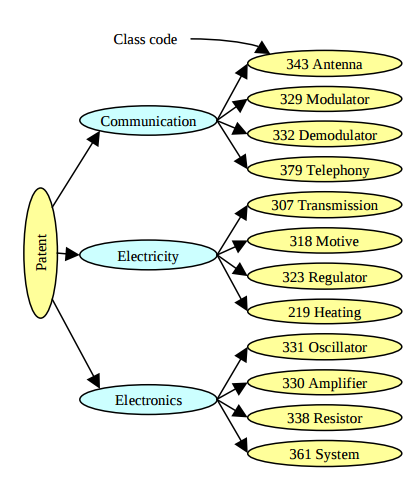
\includegraphics[scale = 0.4]{chakrabarti_1998.png}
%\caption{A topic taxonomy reprinted from Chakrabarti (1998)}\label{fig:chakra}
%\end{figure}

%Cost functions for hierarchical class function are commonly derived
%from graph distances induced by the tree $T$.  For example, one might
%define $C(y', y)$ to be the \emph{graph distance} between $y$ and
%$y'$--that is, the minimal number of edges in the graph for any path
%between $y$ and $y'$.

%[examples of multi-class classifiers? LDA, QDA, OVA, OVO?]

\section{Framework}\label{sec:formulation}

\subsection{Problem Formulation}

This section lays out the basic framework which is necessary to
\emph{formulate} the problem.  However, in the rest of the paper, we
will also adopt some additional assumptions in order to solve the
problem we pose in this section.

Let $\mathcal{Y}$ be a collection of labels and $\mathcal{X}$ be a
space of feature vectors.  For each label $y \in \mathcal{Y}$, there
exists a distribution $F_y$ supported on $\mathcal{X}$.  Also suppose
that there exists a \emph{cost function} $C(\hat{y}, y)$ which
measures the cost of incorrectly labelling an instance as $\hat{y}$
when the correct label is $y$.  Further suppose that $0 \leq C(y, y')
\leq \infty$ and $C(y, y)=0$ for all $y, y' \in \mathcal{Y}$.

A \emph{classification task} consists of a subset of labels,
$\mathcal{S} \subset \mathcal{Y}$, and a prior distribution $\pi$ over
the label subset.  A \emph{classification rule} for the task consists
of a function $f$ which maps feature vectors $x \in \mathcal{X}$ to
labels in $\mathcal{S}$:
\[
f: \mathcal{X} \to \mathcal{S}.
\]
The classification task defines the \emph{risk} of a classification
rule.  Under the classification task, a label $y$ is drawn from the
distribution $\pi$.  Then, we draw $x \sim F_y$.  The label assigned
by the classification rule is $\hat{y} = f(x)$.  The \emph{loss}
incurred is $C(\hat{y}, y)$.  The \emph{risk} of the classification
rule is the expected loss under the class distribution $\pi$:
\[
\text{Risk}(f) = \E_\pi[C(\hat{y}, y)] = \int_\mathcal{S} d \pi(y) \int_{\mathcal{X}} C(f(x), y) dF_y(x).
\]

A \emph{classification model} $\mathcal{F}$ is an algorithm or
procedure for producing classification rules given an empirical
distributions $\hat{F}_y$ for each $y \in \mathcal{S}$, and a vector
of prior probabilities $\pi$.  The model maps a distribution $G$ and a
vector $\pi$ to a classification rule $f$.

We consider \emph{datasets} of size $|\mathcal{S}|r$ for a given
classification task consisting $r$ i.i.d. observations $x_i^{(y)} \sim
F_y$ for each $y \in \mathcal{S}$.  Then define 
\[\hat{F}_y = \frac{1}{r}\sum_{i=1}^r \delta_{x_i^{(y)}}.\]
The sampling distribution of $\hat{F}_y$ is referred to as the
size-$r$ sampling distribution $\Pi_{y, r}$.

The $n$-sample \emph{risk} of the classification model $\mathcal{F}$
is the expected risk of a classification rule $\hat{f} =
\mathcal{F}(\hat{G})$ for a random dataset of size $n$ for the
classification task, $\hat{G} \sim \Pi_n$.  That is,
\[
\text{Risk}_n(\mathcal{F}; \pi) =
\int \text{Risk}(\mathcal{F}(\{\hat{F}_y\}_{y \in \mathcal{S}};
\pi)) \prod_{y \in \mathcal{S}} d\Pi_{y, r}(\hat{F}_y).
\]

The problem of \emph{performance extrapolation} is as follows.
Suppose we have two classification tasks: the $i$th classification
task is specified by label subset $\mathcal{S}_i$, prior distribution
$\pi_i$.  We observe data from the first classification task
consisting of a dataset of size $n_1$.  The goal is to estimate the
$n_2$-sample risk of a $\mathcal{F}$ on the second classification
task, $\text{Risk}_{n_2}(\mathcal{F}; \pi_2)$.

\subsection{Additional assumptions}

In order to obtain a tractable solution to the problem of performance
extrapolation, we make a number of special assumptions on the nature
of the classification tasks, and the classifiers themselves, which
make the problem much easier.

Firstly, we assume that the label space $\mathcal{Y}$ is a continuum:
in fact, that $\mathcal{Y}$ is a subset of $d$-dimensional Euclidean
space. Note this is not such a strong assumption as it might seem,
since cases where there are $k$ discrete labels can be equivalently
formulated as continous models where the the continuum can be
partitioned into $k$ equivalence classes, and in which the cost
between two label $y, y'$ is a function only of their equivalence
classes.

We work with bounded cost functions.  Without loss of generality,
assume that
\[
\sup_{y, y'\in \mathcal{Y}} C(y, y') \leq 1.
\]

With regards to the classification tasks, we assume that there exists
some prior density $\pi_0$ over $\mathcal{Y}$, and that the label
subsets $\mathcal{S}_i = \{y^{(1)}, \hdots, y^{(k_i)}\}$ are obtained
by iid samples with replacement from the density $\nu_0$.  (An
alternative assumption would be that $\mathcal{S}_1 \subset
\mathcal{S}_2$ with $\mathcal{S}_1$ being a subsample of
$\mathcal{S}_2$: this assumption can also be addressed, as we wil
discuss later.)

Next, suppose the prior probabilities for each
classification task are given by
\[
\pi_i(y) = \frac{\pi_0(y)}{\sum_{y' \in \mathcal{S}_i} \pi_0(y')}.
\]
% NOTE: overloading density/distribution pi_0

Further, let us assume that we have more repeats per class in the
first classification task than in the second, $r_1 > r_2$.  We discuss
the possibility of relaxing this condition in the Discussion.

Since the classification tasks are randomly generated, we will aim to
develop a method for estimating the \emph{average risk}.  In the case
where the classification tasks are independently generated, the
average risk is the best predictor (in mean-squared error) for the
(random) risk.

We make some rather strong assumptions with regards to the
classifiers.  The classifier $\mathcal{F}$ produces classification
rules $f$ which depend on \emph{marginal scoring rules}, $m_y$ for $y
\in \mathcal{S}$.  Each marginal scoring rule $m_i$ is a mapping
\[
m_y: \mathcal{X} \to \mathbb{R}.
\]
The classification rule chooses the class with the highest marginal score,
\[
f(x) = \text{argmax}_{y \in \mathcal{S}} m_y(x).
\]
The marginal scoring rules $m_i$, in turn, are generated by a marginal
model $\mathcal{M}$.  The marginal model converts empirical
distributions $\hat{F}$ over $\mathcal{X}$, and an (empirical) prior
class probability, into a marginal scoring function $m: \mathcal{X}
\times \mathbb{R} \to \mathbb{R}$.  For example, one could take 
\[m(x,p) = \log(p) + \log(\hat{f}(x)).\]
where $\hat{f}$ is a density estimate obtained from
$\hat{F}$.  We call such a classification model $\mathcal{F}$ a
\emph{marginal classifier}, and such marginal classifiers are
completely specified by the marginal model $\mathcal{M}.$

Quadratic discriminant analysis and Naive Bayes are two examples of
marginal classification models.
%\footnote{For QDA, the classification function is
%  given by
%\[
%\mathcal{Q}_{QDA}(\hat{F}, y) = -(y - \mu(\hat{F}))^T \Sigma(\hat{F})^{-1} (y-\mu(\hat{F})) - \log\det(\Sigma(\hat{F})),
%\]
%where $\mu(F) = \int y dF(y)$ and $\Sigma(F) = \int (y-\mu(F))(y-\mu(F))^T dF(y)$.
%In Naive Bayes, the classification function is
%\[
%\mathcal{Q}_{NB}(\hat{F},  y) = \sum_{i=1}^n \log \hat{f}_i(y_i),
%\]
%where $\hat{f}_i$ is a density estimate for the $i$-th component of
%$\hat{F}$.}.
The \emph{marginal} property allows us to prove strong results about
the accuracy of the classifier under the exchangeable sampling
assumption, as we see in Section [].

\subsection{Local polynomial regression}

Explain background.

Introduce the notation $\{(w_i, x_i, y_i)\}_{i=1}^n$: ordered triples
of weight, predictor and response.

\subsection{Measurement error models}

Explain background.

\section{Performance extrapolation for marginal classification models}

Having outlined our assumption for randomized label subsets, the focus
of our theory moves towards understanding the $k$-class average risk:
that is, the expected risk of $\mathcal{F}$ when a random subset
$\mathcal{S}$ of size $k$ is drawn.

We obtain a method for estimating the risk in the second
classification task using data from the first.  The insight behind our
estimation method is obtained via an analysis of the average risk of
the classification task.

\subsection{Easy special cases}

Let us first mention two easy special cases, which can be handled
using existing machine learning methodology.

In the special case where $k_1 = k_2 = k$: that is, where the label
subsets $\mathcal{S}_1$ and $\mathcal{S}_2$ are the same size, it is
clear to see that any unbiased estimate of the risk of the classifier
$\mathcal{F}$ for the first classification problem is an unbiased
estimate of the average $k$-class risk.  Since various methods, such
as cross-validation can be used to obtain close-to-unbiased estimates
of the risk in a given classification problem, the problem is
essentially solved for this special case.

Meanwhile, in the case where $k_2 < k_1$, the problem can be solved by
repeatedly subsampling label sets of size $k_2$ from $\mathcal{S}_1$
and averaging unbiased estimates of the risk of each subsampled
classification task.  Aside from computational issues with respect to
computing or approximating the average of ${k_1}\choose{k_2}$
empirical accuracies, the problem is again more or less solved by
using existing methods.

Therefore, the challenging case is when $k_2 > k_1$: we want to
predict the performance of the classification model in a setting with
more labels than we currently see in the training set.

\subsection{Analysis of the average risk}

The average risk is obtained by averaging over four randomizations:
\begin{enumerate}
\item Drawing the label subset $\mathcal{S}$.
\item Drawing the training dataset.
\item Drawing $Y^*$ from $\mathcal{S}$ according to $\pi$.
\item Drawing $X^*$ from $F_{X^*}$.
\end{enumerate}

In other words, one can define a random variable $L$
\[
L = C(\mathcal{F}(\{\hat{F}_y\}_{y \in \mathcal{S}}, \pi)(X^*), Y^*)
\]
which clearly depends on all of the random quantities $\mathcal{S}, \hat{F}_y, \pi, Y^*, X^*$, and where
\[
\text{Average Risk}_k(\mathcal{F}) = \E[L]
\]
where the expectation is taken over all four randomization steps.

As we pointed out in the previous section, the challenging case for
the analysis is the ``undersampled'' regime where we wish to predict
the loss on a larger label set.  Given data with $k_1$ classes, we
already have means to estimate the average risk for all $k \leq k_1$,
so the challenge is to understand how the risk will ``extrapolate'' to
$k > k_1$.  Hence, the goal of the current analysis is to isolate the
effect of $k$, the size of the label subset, on the average risk.

We find that we can do this by \emph{conditioning on} the pair $(x^*,
y^*)$ while \emph{averaging} over the first two steps.
Define the \emph{conditional risk} $R_k(y^*, x^*)$ as
\[
R_k(y^*, x^*) = \E[L|Y^*=y, X^* = x].
\]
Let $G$ denote the joint distribution over $(X, Y)$ obtained by
drawing $Y \sim \pi_0$ and $X \sim F_Y$.  Since $Y^*$ has the marginal
distribution $\pi_0$, it follows that
\begin{equation}\label{eq:rk_eq}
\text{Average Risk}_k(\mathcal{F}) = \int \int R_k(y^*, x^*) dG(x^*, y^*).
\end{equation}
What we have done is to rewrite the average risk as the expectation of
$R_k$, which depends on $k$, according to a measure $G$ which does
\emph{not} depend on $k$.

However, we will further decompose $R_k$ into $k$-dependent and $k$-independent components.

Additional technical assumptions:
\begin{itemize}
\item 
Scaling property of margins, if $\mathcal{M}(\hat{F}_1, \pi_1)(x) >
\mathcal{M}(\hat{F}_2, \pi_2)(x)$ then also $\mathcal{M}(\hat{F}_1,
c\pi_1)(x) > \mathcal{M}(\hat{F}_2, c\pi_2)(x)$.
\item 
Tie-breaking condition, for all $x \in \mathcal{X}$,
$\mathcal{M}(\hat{F}_1, \pi_1)(x) = \mathcal{M}(\hat{F}_2, \pi_2)(x)$
with zero probability.
\end{itemize}

Define the U-functions
\begin{align}\label{eq:ufunc}
U_x(y) &= \Pr[\mathcal{F}(\hat{F}_y, \pi_0(y))(x) > \mathcal{F}(\hat{F}_Y, \pi_0(Y))(x)]
\\&= \int_{\mathcal{Y}} 
I\{
\mathcal{F}(\hat{F}_y, \pi_0(y))(x) > \mathcal{F}(\hat{F}_{y'}, \pi_0(y'))(x)
\}
d\Pi_{y, r}(\hat{F}_y)
d\Pi_{y', r}(\hat{F}_{y'})
d\pi_0(y').
\end{align}
Under the scaling property of margins, we have
\[
U_x(y) =  \Pr[\mathcal{F}(\hat{F}_y, \pi(y))(x) > \mathcal{F}(\hat{F}_Y, \pi(Y))(x)]
\]
for the \emph{random} $\pi$ corresponding to $\mathcal{S}$.  Hence,
$U_x(y)$ gives the probability that an observation $x$ would be
assigned to class $y$, supposing that the only two choices for labels
were $y$ and $Y'$, with $Y'$ drawn uniformly from $\pi_0$.

Note that the random variable $U_x(Y)$ for $Y \sim \pi_0$ is uniformly
distributed for all $x \in \mathcal{X}$ (hence the name ``U-function'').

%And, under the tie-breaking condition, we have
%\[
%R_k(y^*, x^*) = \int U_{x^*}(y)^{k-2} I\{U_{x^*}(y) > U_{x}(y^*)\} C(y, y^*) d\pi_0(y).
%\]
%This integral expression can be further re-written in order to isolate the dependence on $k$.
Define the \emph{conditional cost function} $K(y^*, x^*, u)$ by
\begin{equation}\label{eq:Kfunc}
K(y^*, x^*, u) = \mathbb{E}[C(Y, y^*)I\{U_{x^*}(Y) > U_{x^*}(y^*)\}|U_{x^*}(y) = u].
\end{equation}
The conditional cost function gives the expected cost conditional on
$x^*, y^*$, and the $U_{x^*}$-value of the incorrect label with the
largest margin.

Obtaining the conditional risk $R_k(y^*, x^*)$ from the conditional
cost function requires the following observation.  Let the $(k-1)$
incorrect labels in $\mathcal{S}$ be denoted by $y^{(1)},\hdots,
y^{(k-1)}$, and define $U_i = U_{X^*}(y^{(i)})$. Let $U_{max}$ denote the $U_{x^*}$-value of
the incorrect label: we have
\[
U_{max} = \max_{i=1}^{k-1} U_i.
\]
Meanwhile, by definition, we have
\[
R_k(y^*, x^*) = \E[K(y^*, x^*, U_{max})].
\]
But we know the density of $U_{max}$!  Recall that $U_i$ are iid
uniform, and therefore $U_{max}$ has density $p(u) = ku^{k-1}$.  We
therefore have
\[
R_k(y^*, x^*) = k \int K(y^*, x^*, u) u^{k-1} du.
\]

Returning to equation \eqref{eq:rk_eq}, we obtain
\[
\text{Average Risk}_k(\mathcal{F}) = k \int u^{k-1} du \int K(y^*, x^*, u) dG(x^*, y^*) = k \int u^{k-1} \bar{K}(u) du,
\]
where
\begin{equation}\label{eq:Kbar}
\bar{K}(u) = \int K(y^*, x^*, u) dG(x^*, y^*).
\end{equation}
The average risk is expressed as a weighted integral of a certain
function $\bar{K}(u)$ defined on $u \in [0,1]$.  We have clearly
isolated the part of the average risk which is independent of $k$--the
univariate function $\bar{K}(u)$, and the part which is dependent on
$k$--which is the weighting density $ku^{k-1}$ (which is the
Beta($k$, 1) density.)

This is the key result behind our estimation method, and we restate it
in the following theorem.

\begin{theorem}
Suppose $\pi$, $\{F_y\}_{y \in \mathcal{Y}}$ and marginal classifier
$\mathcal{F}$ satisfy the marginal scaling condition tie-breaking
condition.  Then, under the definitions \eqref{eq:ufunc}, \eqref{eq:Kfunc}, and \eqref{eq:Kbar}, we have
\begin{equation}\label{eq:avrisk_identity}
\text{AvRisk}_k(\mathcal{F}) = k \int u^{k-1} \bar{K}(u) du.
\end{equation}
\end{theorem}

The proof is given in the appendix.

Having this theoretical result allows us to understand how the
expected $k$-class risk scales with $k$ in problems where all the
relevant densities are known.  However, applying this result in
practice to estimate $\text{Average Risk}_k$ requires some means of
estimating the unknown function $\bar{K}$--which we discuss in the
following.

\subsection{Estimation}

Now we address the problem of estimating $\text{Average Risk}_{k_2}$
from data.  

First, let us assume a $d$-th order polynomial model
\[
\bar{K}(u) = \sum_{\ell = 0}^d \beta_\ell u^\ell.
\]

Recall that the data consists of $k_1 < k_2$ classes, with
$r_1$ repeats per class.  The set of class labels is $\mathcal{S}_1 =
\{y^{(1)},\hdots, y^{(k_1)}\}$.  For each class $i = 1,\hdots, k_1$,
we have repeats $x_j^{(i)}$ for $j = 1,\hdots, r_1$.

Define $r_{test} = r_1 - r_2$.  Let us take the first $r_{test}$
repeats per class, and form the \emph{test set} $\{x_j^{(i)}\}_{j=1,
  i=1}^{r_{test}, k_1}$.  From the remaining $r_2$ repeats, we form
the empirical distributions
\[
\hat{F}_{y^{(i)}} = \frac{1}{r_2}\sum_{j=r_{test} + 1}^{r_1} \delta_{x_j^{(i)}}.
\]
The marginal model $\mathcal{M}$ yields margins for each point in the
test set for each label in $\mathcal{S}_1$.  Define the margins
\[
M_{i, j}^\ell = \mathcal{M}(\hat{F}_{y^{(\ell)}}; \pi_1(y^{(\ell)}))(x_j^{(i)}).
\]
The predicted label for each test point is
\[
\hat{y}_{i,j} = y^{(\argmax_{\ell \in \{1,\hdots, k\}} M_{i, j}^\ell)}.
\]
Therefore, an unbiased estimate of the risk (which is also an unbiased
estimate of the $k_1$-class average risk) is
\[
\text{Test Risk} = \frac{1}{r_{test}}\sum_{i=1}^k \sum_{j=1}^{r_{test}} \frac{\pi_0(y^{(i)})}{\nu_0(y^{(i)})} C(\hat{y}_{i, j}, y^{(i)}).
\]

Now we turn to the question of estimating the function $\bar{K}(u)$.
Suppose that hypothetically, we could have observed the quantities
$U_{i, j, \ell}$, defined
\[
U_{i, j, \ell} = U_{x_j^{(i)}}(y^{(\ell)}).
\]
Also define
\[
C_{i,\ell} = C(y^{(\ell)}, y^{(i)})
\]
and
\[
w_i = \frac{\pi_0(y^{(i)})}{\nu_0(y^{(i)})}.
\]
Then $\bar{K}(u)$ could be estimated via a $d$-th order polynomial regression
\[
\hat{\beta} = \argmin_{\beta} \sum_{i=1,j=1, \ell=1}^{r_{test}, k_1, k_1} w_i \left(C_i^\ell - \sum_{h=0}^d \beta_h U_{i,j, \ell}^d\right)^2
\]
for the
dataset $\{(w_i, U_{i,j, \ell}, C_{i,\ell})\}_{i=1, j=1,
  \ell=1}^{r_{test}, k_1, k_1}$.  However, this is not possible in
practice because $U_{i,j,\ell}$ are not directly observed.

Instead, we can obtain unbiased estimates via
\[
\hat{U}_{i,j, \ell} = \frac{1}{(k-1)\zeta}\sum_{m \neq \ell}  \frac{\pi_0(y^{(m)})}{\nu_0(y^{(m)})} I\{M_{i, j}^\ell > M_{i, j}^m\}
\]
However, if we were to simply treat $\hat{U}_{i, j, \ell}$ as a proxy
for the unobserved $U_{i,j,\ell}$, and apply polynomial regression to
the dataset
\[
\{(w_i, \hat{U}_{i,j, \ell}, C_{i, \ell})\}_{i=1, j=1, \ell=1}^{r_{test}, k_1,k_1},
\]
the estimated $\widehat{\bar{K}(u)}$ would be biased, since we have
\emph{errors-in-covariates}.  It is necessary to make use of the
\emph{covariate adjustment} technique.  Covariate adjustment is
justified since the error in the covariates is conditionally
independent of the response given the true covariates:
\[
\hat{U}_{i,j,\ell} \perp C_i^\ell | U_{i, j,\ell}.
\]

In the naive polynomial regression, the predictors are the powers of
the unbiased estimates, $\hat{U}_{i,j,\ell}^h$ for $h = 0,\hdots, d$.
The issue is that while $\hat{U}_{i,j,\ell}$ is unbiased for
$U_{i,j,\ell}$, the higher powers of $\hat{U}_{i,j,\ell}$ are
\emph{not} unbiased estimators of the higher powers of $U_{i,j,\ell}$.
Covariate adjustment in this case amounts to replacing the naive
estimates $\hat{U}_{i,j,\ell}^h$ with unbiased estimators.

% reconfigure notation to get rid of indicators somehow??
There exist U-statistic estimators of the higher powers of
$\hat{U}_{i,j,\ell}^h$.  For instance, for $h=2$, the estimator is
\[
\hat{U}_{i,j,\ell}^{(2)} = \frac{1}{\zeta^2 k(k-1)} \sum_{m_1\neq m_2 \neq j}  \frac{\pi_0(y^{(m_1)})}{\nu_0(y^{(m_2)})} I\{M_{i, j}^\ell > M_{i, j}^{m_2}\}
 \frac{\pi_0(y^{(m_2)})}{\nu_0(y^{(m_2)})} I\{M_{i, j}^\ell > M_{i, j}^{m_2}\}.
\]
In general, the U-statistic is
\[
\hat{U}_{i, j, \ell}^{(h)} = \frac{(k-h)!}{\zeta^h k!} \sum_{m_1 \neq \cdots \neq m_h \neq j} \prod_{z=1}^h  \frac{\pi_0(y^{(m_z)})}{\nu_0(y^{(m_z)})} I\{M_{i, j}^\ell > M_{i, j}^{m_z}\}.
\]

In summation, the algorithm is as follows:
% summary of algorithm

\subsection{Monotonicity assumption}

Assuming that $\bar{K}(u)$ in monotone in $u \in [0,1]$.
Justification and implications.

\section{Special case: uniform prior and zero-one loss}

For the special case of zero-one loss and uniform prior, the theory
becomes simplified and additional methods of estimation are possible.

Define
\[
\gamma_m = \int_0^1 \bar{K}(u)  \frac{k_1!}{(m-1)!(k_1-m)!} u^{m-1} (1-u)^{k_1-m} du
\]
for $m = 1,\hdots, k_1$.

Define the \emph{ranks}
\[
R_{i, j, \ell} = (k-1)\hat{U}_{i, j, \ell}.
\]
Due to the uniform prior, $R_{ij}^\ell \in \{0,\hdots, k_1-1\}$.

Define
\[
C_{ij}^{(h)} = \sum_{\ell=1}^k I\{R_{i, j, \ell} = h - 1\} C_{i, \ell},
\]
i.e., the cost incurred for the class with the $h$th smallest rank for
the observation $x_i^{(\ell)}$.

Note that the test risk for $k_1$ classes can be written as
\[
\text{Test Risk}_k = \frac{1}{r_{test}k_1}\sum_{i=1,j=1}^{k_1,r_{test}} C_{ij}^{(k_1)}.
\]

Since $C_{ij}^\ell$ is now a binary random variable, we have
\[
C_{ij}^{(h)} \sim \text{Bernoulli}(\gamma_h).
\]

If $C_{ij}^{(h)}$ were independent, one could estimate $\gamma_h$ by
maximizing the log-likelihood
\begin{equation}\label{eq:pseudolikelihood1}
\mathcal{L}(\vec{\gamma}) = \sum_{i=1,j=1,h=1}^{k_1, r_{test}, k_1} C_{ij}^{(h)} \log \gamma_h + (1-C_{ij})^{(h)} \log (1-\gamma_h)
\end{equation}

However, since $C_{ij}^{(h)}$ are not independent, the equation
\eqref{eq:pseudolikelihood1} is not a likelihood, but a
\emph{pseudolikelihood}.  Nevertheless, one can attempt to estimate
$\gamma_h$ using the method.

The basic idea of using pseudolikelihood leads to many different
practical approaches for estimating the average $k$-class risk.  We tried the following approaches:
\begin{enumerate}
\item Estimate unconstrained $\gamma_h$, then find a function
  $\bar{K}(u)$ which satisfies the moment constraints implied by the
  estimates $\hat{\gamma}_h$.  Estimate $\text{AvgRisk}_k$ by plugging
  in the estimated $\hat{K}(u)$ into \eqref{eq:avrisk_identity}.
\item Let $\hat{K}(u)$ be constrained by the test risk (which is unbiased for the $k_1$-class average risk,)
\[
\text{Test Risk}_l = \int_0^1 \hat{K}(u) k_1 u^{k_1 -1} du.
\]
Under this moment constraint, estimate $\hat{K}(u)$ using pseudolikelihood.
%needs to be clarified how pseudolikelihood can be used to estimate either hatKu or gamma
\item Either of the above two approaches, plus a monotonicity constraint on $\hat{K}(u).$
\end{enumerate}




\end{document}





Define
\[
\bar{C}_m = \frac{1}{r_{test}}\sum_{j=1}^{r_{test}} \sum_{j=1, i=1, \ell = 1}^{r_{test}, k_1, k_1} C_i^\ell I\{\hat{U}_{ij}^\ell = \frac{m-1}{k_1-1}\}
\]
for $m = 1,\hdots, k_1$, and let $\vec{C} = (\bar{C}_1,\hdots,
\bar{C}_k)$.

We have
\[
\E[\bar{C}_m] = \int_0^1 K(u) \frac{k_1!}{(m-1)!(k_2-m)!} u^{m-1} (1-u)^{k_1-m}  du,
\]
and the approximate variance upper bound
\[
v_m = \Var[\bar{C}_m] \lessapprox \frac{\bar{C}_m (1-\bar{C})_m}{r}.
\]
under the assumption that $\sup_{\mathcal{Y}^2} C(y, y') \leq 1$.

Now suppose we adopt a linear model
\[
\bar{K}(u) = \sum_{\ell=1}^d \beta_\ell h_\ell(u)
\]
where $h_\ell(u)$ are some basis functions.
If we knew $\beta_\ell$, then we could determine the average risk for any $k$, since
defining
\[
W_\ell = \int_0^1 h_\ell(u) K u^{K-1} du.
\]
we have
\begin{equation}\label{eq:avgrisk_linmod}
\text{AvRisk}_k(\mathcal{F}) = \int_0^1 \bar{K}(u) k u^{k-1} du = \sum_{\ell=1}^d \beta_\ell W_\ell.
\end{equation}



Then it follows that
defining
\[
Z_{m, \ell} = \int_0^1 h_\ell(u) \frac{k!}{(m-1)!(k-m)!} u^{m-1} (1-u)^{k-m} du
\]
for $\ell = 1,\hdots, d$, we have
\[
\E[\bar{C}_m] = \sum_{\ell = 1}^d \beta_\ell Z_{m, \ell}.
\]
Therefore, we can apply linear regression to the dataset
\[
\{(v_m, \vec{Z}_m, \bar{C}_m)\}
\]
where $\vec{Z}_m = (Z_{m, 1},\hdots, Z_{m, d})$,
obtaining the coefficient estimate
\[
\hat{\beta} = (\bZ^T V^{-1} \bZ)^{-1} \bZ^T V^{-1} \vec{C},
\]
where the matrices $\bZ = (Z_{m, \ell})$ and $V =
\text{diag}(v_1,\hdots, v_k)$.

Now we can consider prediction of the average risk.
Plugging in the estimates of $\beta$ into \eqref{eq:avgrisk_linmod}, we get the unbiased risk estimate
\[
\widehat{AvRisk}_k(\mathcal{F}) = \hat{\beta}^T \vec{W},
\]
where $\vec{W} = (W_1,\hdots, W_d)$.
The variance of the estimate is approximately bounded by
\[
\Var[\widehat{AvRisk}_k(\mathcal{F})] \lessapprox \vec{W}^T (\bZ^T V^{-1} \bZ)^{-1} \vec{W}.
\]



\end{document}





\subsection{Convergence analysis}



Taking a fairly conservative analysis, we will use the universal variance bound
\[
\Var[\bar{C}_m] \leq \frac{1}{4r}
\]
which holds given the condition $\sup_{\mathcal{Y}^2} C(y, y') \leq 1.$

We have the explicit formulas
\[
W_\ell = \frac{\ell!(K-\ell)!}{K!}
\]
and
\[
Z_{m, \ell} = \frac{(m+\ell-1)!(k-1)!}{(m-1)!(k+\ell-1)!}.
\]

The variance of the unbiased estimate of average risk is bounded by
\[
\Var[\widehat{AvRisk}_k(\mathcal{F})] \leq \frac{1}{4r} \vec{W}^T (\bZ^T \bZ)^{-1} \vec{W}.
\]
The bound depends only on the quantities $r, d, k, K$, and can be
easily computed numerically.  However, it is easy to see that in the
$r \to \infty$ limit, consistent estimation results.  It remains to
understand how the asymptotic performance of our estimation procedure
depends on the parameters $d, k, K$.

Define
\[
\kappa(k, K, d) = \vec{W}^T (\bZ^T \bZ)^{-1} \vec{W}.
\]

























In multi-class classification, one observes pairs $(z, y)$ where $y
\in \mathcal{Y} \subset \mathbb{R}^p$ are feature vectors, and $z$ are
unknown labels, which lie in a countable label set $\mathcal{Z}$.  The
goal is to construct a classification rule for predicting the label of
a new data point; generally, the classification rule $h: \mathcal{Y}
\to \mathcal{Z}$ is learned from previously observed data points.  In
many applications of multi-class classification, such as face
recognition or image recognition, the space of potential labels is
practically infinite.  In such a setting, one might consider a
sequence of classification problems on finite label subsets
$\mathcal{Z}_1 \subset \cdots \subset \mathcal{Z}_K$, where in the
$i$-th problem, one constructs the classification rule
$h^{(i)}:\mathcal{Y} \to \mathcal{Z}_i$.  Supposing that $(Z, Y)$ have
a joint distribution, define the accuracy for the $i$-th problem as
\[
\text{acc}^{(i)} = \Pr[h^{(i)}(Y) = Z|Z \in \mathcal{Z}_i].
\]
Using data from only $\mathcal{Z}_k$, can one predict the accuracy achieved on the larger label set $\mathcal{Z}_K$, with $K> k$?  This is the problem of \emph{performance extrapolation}.

A practical instance of performance extrapolation occurs in
neuroimaging studies, where the number of classes $k$ is limited by
experimental considerations.  Kay et al. [1] obtained fMRI brain scans
which record how a single subject's visual cortex responds to natural
images.  The label set $\mathcal{Z}$ corresponds to the space of all
grayscale photographs of natural images, and the set $\mathcal{Z}_1$
is a subset of 1750 photographs used in the experiment.  They
construct a classifier which achieves over 0.75 accuracy for
classifying the 1750 photographs; based on exponential extrapolation,
they estimate that it would take on the order of $10^{9.5}$
photographs before the accuracy of the model drops below 0.10!
Directly validating this estimate would take immense resources, so it
would be useful to develop the theory needed to understand how to
compute such extrapolations in a principled way.

However, in the fully general setting, it is impossible on construct
non-trivial bounds on the accuracy achieved on the new classes
$\mathcal{Z}_K \setminus \mathcal{Z}_k$ based only on knowledge of
$\mathcal{Z}_k$: after all, $\mathcal{Z}_k$ could consist entirely of
well-separated classes while the new classes $\mathcal{Z}_K \setminus
\mathcal{Z}_k$ consist entirely of highly inseparable classes, or
vice-versa.  Thus, the most important assumption for our theory is
that of \emph{exchangeable sampling}.  The labels in $\mathcal{Z}_i$
are assumed to be an exchangeable sample from $\mathcal{Z}$.  The
condition of exchangeability ensures that the separability of random
subsets of $\mathcal{Z}$ can be inferred by looking at the empirical
distributions in $\mathcal{Z}_k$, and therefore that some estimate of
the achievable accuracy on $\mathcal{Z}_K$ can be obtained.

The assumption of exchangeability greatly limits the scope of
application for our methods.  Many multi-class classification problems
have a hierarchical structure [2], or have class labels distributed
according to non-uniform discrete distributions, e.g. power laws [3];
in either case, exchangeability is violated.  It would be interesting
to extend our theory to the hierarchical setting, or to handle
non-hierarchical settings with non-uniform prior class probabilities,
but again we leave the subject for future work.

In addition to the assumption of exchangeability, we consider a
restricted set of classifiers.  We focus on \emph{generative
  classifiers}, which are classifiers that work by training a model
separately on each class.  This convenient property allows us to
characterize the accuracy of the classifier by selectively
conditioning on one class at a time.  In section 3, we use this
technique to reveal an equivalence between the expected accuracies of
$\mathcal{Z}_k$ to moments of a common distribution.  This moment
equivalence result allows standard approaches in statistics, such as
U-statistics and nonparametric pseudolikelilood, to be directly
applied to the extrapolation problem, as we discuss in section 4.  In
non-generative classifiers, the classification rule has a joint
dependence on the entire set of classes, and cannot be analyzed by
conditioning on individual classes.  In section 5, we empirically
study the performance of our classifiers.  Since generative
classifiers only comprise a minority of the classifiers used in
practice, we applied our methods to a variety of generative and
non-generative classifiers in simulations and in one OCR dataset.  Our
methods have varying success on generative and non-generative
classifiers, but seem to work badly for neural networks.

\noindent\emph{Our contribution.}

To our knowledge, we are the first to formalize the problem of
prediction extrapolation.  We introduce three methods for prediction
extrapolation: the method of extended unbiased estimation and the
constrained pseudolikelihood method are novel.  The third method,
based on asymptotics, is a new application of a recently proposed
method for estimating mutual information [4].

\section{Setting}

Having motivated the problem of performance extrapolation, we now
reformulate the problem for notational and theoretical convenience.
Instead of requiring $\mathcal{Z}_k$ to be a random subset of
$\mathcal{Z}$ as we did in section 1, take $\mathcal{Z}=\mathbb{N}$
and $\mathcal{Z}_k = \{1,\hdots, k\}$.  We fix the size of
$\mathcal{Z}_k$ without losing generality, since any monotonic
sequence of finite subsets can be embedded in a sequence with
$|\mathcal{Z}_k| = k$.  In addition, rather than randomizing the
labels, we will randomize the marginal distribution $p(y|z)$ of each
label; Towards that end, let $\mathcal{Y} \subset \mathbb{R}^p$ be a
space of feature vectors, and let $\mathcal{P}(\mathcal{Y})$ be a
measurable space of probability distributions on $\mathcal{Y}$.  Let
$\mathbb{F}$ be a probability measure on $\mathcal{P}$, and let $F_1,
F_2,\hdots$ be an infinite sequence of i.i.d. draws from $\mathbb{F}$.
We refer to $\mathbb{F}$, a probability measure on probability
measures, as a \emph{meta-distribution}.  The distributions
$F_1,\hdots, F_k$ are the marginal distributions of the first $k$
classes.  Further assuming that the labels are equiprobable, we
rewrite the accuracy as
\[
\text{acc}^{(t)} = \frac{1}{t}\sum_{i=1}^t \Pr_{F_i}[h^{(t)}(Y) = i].
\]
where the probabilities are taken over $Y \sim F_i$.

In order to construct the classification rule $h^{(t)}$, we need data from the classes $F_1,\hdots, F_t$.
In most instances of multi-class classification, one observes independent observations from each $F_i$
which are used to construct the classifier.  Since the order of the observations
does not generally matter, a sufficient statistic for the training data for the $t$-th classification problem
is the collection of empirical distributions
$\hat{F}_1^{(t)},\hdots,\hat{F}_t^{(t)}$ for each class.
Henceforth, we make the simplifying assumption that the training data for the $i$-th class remains fixed
from $t =i, i+1,\hdots$, so we drop the superscript on $\hat{F}_i^{(t)}$.
Write $\hat{\mathbb{F}}(F)$ for the conditional distribution of $\hat{F}_i$ given  $F_i = F$;
also write $\hat{\mathbb{F}}$ for the marginal distribution of $\hat{F}$ when $F \sim \mathbb{F}.$
As an example, suppose every class has the number of training examples $r \in \mathbb{N}$; then $\hat{F}$
is the empirical distribution of $r$ i.i.d. observations from $F$, and $\hat{\mathbb{F}}(F)$ is the \emph{empirical meta-distribution} of $\hat{F}$.
Meanwhile, $\hat{\mathbb{F}}$ is the true meta-distribution of the empirical distribution of $r$ i.i.d. draws from a random $F \sim \mathbb{F}$.


\subsection{Multiclass classification}

Extending the formalism of Tewari and Bartlett [5]\footnote{As in
  their framework, we define a classifier as a vector-valued function.
  However, we introduce the notion of a classifier as a
  multiple-argument functional on empirical distributions, which
  echoes the functional formulation of estimators common in the
  statistical literature.}, we define a classifier as a collection of
mappings $\mathcal{M}_i: \mathcal{P}(\mathcal{Y})^k \times \mathcal{Y}
\to \mathbb{R}$ called \emph{classification functions.}  Intuitively
speaking, each classification function \emph{learns a model} from the
first $k$ arguments, which are the empirical marginals of the $k$
classes, $\hat{F}_1,\hdots, \hat{F}_k$.  For each class, the
classifier assigns a real-valued \emph{classification score} to the
\emph{query point} $y \in \mathcal{Y}$.  A higher score
$\mathcal{M}_i(\hat{F}_1,\hdots, \hat{F}_k, y)$ indicates a higher
estimated probability that $y$ belongs to the $k$-th class.
Therefore, the classification rule corresponding to a classifier
$\mathcal{M}_i$ assigns a class with maximum classification score to
$y$:
\[
h(y) = \argmax_{i \in \{1,\hdots, k\}} \mathcal{M}_i(y).
\]
For some classifiers, the classification functions $\mathcal{M}_i$ are especially simple
in that $\mathcal{M}_i$ is only a function of $\hat{F}_i$ and $y$.
Furthermore, due to symmetry, in such cases one can write
\[
\mathcal{M}_i(\hat{F}_1,\hdots, \hat{F}_k, y) = \mathcal{Q}(\hat{F}_i, y),
\]
where $\mathcal{Q}$ is called a \emph{single-class classification function} (or simply \emph{classification function}),
and we say that $\mathcal{M}$ is a \emph{generative classifier}.
Quadratic discriminant analysis and Naive Bayes [6] are two examples of
generative classifiers\footnote{For QDA, the classification function is given by
\[
\mathcal{Q}_{QDA}(\hat{F}, y) = -(y - \mu(\hat{F}))^T \Sigma(\hat{F})^{-1} (y-\mu(\hat{F})) - \log\det(\Sigma(\hat{F})),
\]
where $\mu(F) = \int y dF(y)$ and $\Sigma(F) = \int (y-\mu(F))(y-\mu(F))^T dF(y)$.
In Naive Bayes, the classification function is
\[
\mathcal{Q}_{NB}(\hat{F},  y) = \sum_{i=1}^n \log \hat{f}_i(y_i),
\]
where $\hat{f}_i$ is a density estimate for the $i$-th component of
$\hat{F}$.}.
The \emph{generative} property allows us to prove strong results about the accuracy of the classifier
under the exchangeable sampling assumption, as we see in Section 3.

\section{Performance extrapolation for generative classifiers}

Let us specialize to the case of a generative classifier, with classification function $\mathcal{Q}$.
Consider estimating the expected accuracy for the $k$-th classification problem,
\begin{equation}\label{eq:pt}
p_k \stackrel{def}{=} \E[\text{acc}^{(k)}].\end{equation}
In the case of a generative classifier, we have
\[
p_k = \E[acc^{(k)}] = \E\left[\frac{1}{k}\sum_{i=1}^k \Pr_{Y \sim F_i}[\mathcal{Q}(\hat{F}_i, Y) > \max_{j \neq i}\mathcal{Q}(\hat{F}_j, Y)]\right].
\]
Define the \emph{conditional accuracy} function $u(\hat{F}, y)$ which maps a
distribution $\hat{F}$ on $\mathcal{Y}$ and a \emph{test} observation $y$ to
a real number in $[0,1]$.  The conditional accuracy gives the
probability that for independently drawn $\hat{F}'$ from $\hat{\mathbb{F}}$, that
$\mathcal{Q}(\hat{F}, y)$ will be greater than $\mathcal{Q}(\hat{F}', y)$:
\[
u(\hat{F}, y) = \Pr_{\hat{F}' \sim \hat{\mathbb{F}}}[\mathcal{Q}(\hat{F}, y) > \mathcal{Q}(\hat{F}', y)].
\]
Define the \emph{conditional accuracy} distribution $\nu$ as the law
of $u(\hat{F}, Y)$ where $\hat{F}$ and $Y$ are generated as follows:
(i) a true distribution $F$ is drawn from $\mathbb{F}$; 
(ii) the empirical distribution $\hat{F}$ is drawn from $\hat{\mathbb{F}}(F)$ (i.e., the training data for the class),
(iii) the query $Y$ is drawn from $F$, with $Y$ independent of $\hat{F}$ (i.e. a single test data point from the same class.)
The significance of the conditional accuracy
distribution is that the expected accuracy $p_t$ can be
written in terms of its moments.

\noindent\textbf{Theorem 3.1.} \emph{
Let $\mathcal{Q}$ be a single-distribution classification function, and let $\mathbb{F}$, $\hat{\mathbb{F}}(F)$ be a distribution on $\mathcal{P}(\mathcal{Y}).$
Further assume that
$\hat{\mathbb{F}}$ and $\mathcal{Q}$ jointly satisfy the
\emph{tie-breaking} property:
\begin{equation}\label{eq:tie}
\Pr[\mathcal{Q}(\hat{F}, y) = \mathcal{Q}(\hat{F}', y)] = 0
\end{equation}
for all $y \in \mathcal{Y}$, where $\hat{F}, \hat{F}' \stackrel{iid}{\sim} \hat{\mathbb{F}}$.
Let $U$ be defined as the random variable
$U = u(\hat{F}, Y)$
for $F \sim \mathbb{F}$, $Y \sim F$, and $\hat{F} \sim \hat{\mathbb{F}}(F)$ with $Y \perp \hat{F}$.
Then \[p_k = \E[U^{k-1}],\]
where $p_k$ is the expected accuracy as defined by \eqref{eq:pt}.
}

(Proof is included in the supplement.)

%\noindent\textbf{Proof.}  
%Write $q^{(i)}(y) = \mathcal{Q}(\hat{F}_i, y)$.
%By using conditioning and
%conditional independence, $p_k$ can be written
%\begin{align*}
%p_k &= \E\left[ \frac{1}{k}\sum_{i=1}^k  \Pr_{F_i}[q^{(i)}(Y) > \max_{j\neq i} q^{(j)}(Y)] %\right]
%\\&= \E\left[ \Pr_{F_1}[q^{(1)}(Y) > \max_{j\neq 1} q^{(j)}(Y)] \right]
%\\&= \E_{F_1}[\Pr[q^{(1)}(Y) > \max_{j\neq 1} q^{(j)}(Y)|\hat{F}_1, Y]]
%\\&= \E_{F_1}[\Pr[\cap_{j > 1} q^{(1)}(Y) > q^{(j)}(Y)|\hat{F}_1, Y]]
%\\&= \E_{F_1}[\prod_{j > 1}\Pr[q^{(1)}(Y) > q^{(j)}(Y)|\hat{F}_1, Y]]
%\\&= \E_{F_1}[\Pr[q^{(1)}(Y) > q^{(2)}(Y)|\hat{F}_1, Y]^{k-1}]
%\\&= \E_{F_1}[u(\hat{F}_1, Y)^{k-1}] = \E[U^{k-1}].
%\end{align*}
%$\Box$

Theorem 3.1 tells us that the problem of extrapolation can be
approached by attempting to estimate the conditional accuracy
distribution.  The $(t-1)$-th moment of $U$ gives us $p_t$, which will
in turn be a good estimate of $\text{acc}^{(t)}$.

While $U = u(\hat{F}, Y)$ is not directly observed, we can obtain unbiased estimates of $u(\hat{F}_i, y)$
by using test data.  For any $\hat{F}_1,\hdots, \hat{F}_k$, and independent test point $Y \sim F_i$, define
\begin{equation}\label{eq:hatu}
\hat{u}(\hat{F}_i, Y) = \frac{1}{k -1}\sum_{j \neq i} I(\mathcal{Q}(\hat{F}_i, Y) > \mathcal{Q}(\hat{F}_j, Y)).
\end{equation}
Then $\hat{u}(\hat{F}_i, Y)$ is an unbiased estimate of $u(\hat{F}_i, Y)$, as stated in the following theorem.

\noindent\textbf{Theorem 3.2.}\emph{
Assume the conditions of theorem 3.1.
Then defining 
\begin{equation}\label{eq:veq}
V = (k-1)\hat{u}(\hat{F}_i, y),\end{equation}
we have
\[V \sim \text{\emph{Binomial}}(k-1, u(\hat{F}_i, y)).\]
Hence,
\[\E[\hat{u}(\hat{F}_i, y)] = u(\hat{F}_i, y).\]
}

In section 4, we will use this result to estimate the moments of $U$.
Meanwhile, since $U$ is a random variable on $[0, 1]$, we also conclude that $p_t$ follows a \emph{mixed exponential decay}.
Let $\alpha$ be the law of $-\log(U)$.
Then from change-of-variables $\kappa =-\log(u)$, we get
\[p_t = \E[U^{t-1}] = 
\int_0^1 u^{t-1} d\nu(u) = \int_0^1 e^{t\log(u)} \frac{1}{u}d\nu(u) = 
\int_{\mathbb{R}^{+}} e^{-\kappa t} d\alpha(\kappa).\]
This fact immediately suggests the technique of fitting a mixture of exponentials to the test accuracy at $t =2,3,\hdots, k$:
we explore this idea further in Section 4.1.

\subsection{Properties of the conditional accuracy distribution}

The conditional accuracy distribution $\nu$ is determined by $\mathbb{F}$
and $\mathcal{Q}$.  What can we say about the the conditional accuracy
distribution without making any assumptions on either $\mathbb{F}$ or
$\mathcal{Q}$?  The answer is: not much.  For an arbitrary probability
measure $\nu'$ on $[0,1]$, one can construct $\mathbb{F}$ and
$\mathcal{Q}$ such that the conditional accuracy $U$ has the distribution $\nu'$, even if one makes the \emph{perfect sampling assumption} that $\hat{F}=F.$

\noindent\textbf{Theorem 3.3.} \emph{ Let $U$ be defined as in Theorem
  3.1, and let $\nu$ denote the law of $U$.  Then, for any probability
  distribution $\nu'$ on $[0,1]$, one can construct a
  meta-distribution $\mathbb{F}$ and a classification function $\mathcal{Q}$ such
  that the conditional accuracy $U$ has distribution $\nu'$ under perfect sampling (that is, $\hat{F} = F$.)  }

\textbf{Proof.}  
Let $G$ be the cdf of $\nu$, $G(x) = \int_0^x d\nu(x)$, and let $H(u) = \sup_x \{G(x) \leq u\}$.
Define $\mathcal{Q}$ by
\[
\mathcal{Q}(\hat{F}, y) = \begin{cases}
0 &\text{ if }\mu(\hat{F}) > y + H(y)\\
0 & \text{ if }y + H(y) > 1 \text{ and }\mu(\hat{F}) \in [H(y) - y, y]\\
1 + \mu(\hat{F}) - y &\text{ if } \mu(\hat{F}) \in [y, y + H(y)]\\
1 + y + \mu(\hat{F}) &\text{ if }\mu(\hat{F}) + H(y) > 1 \text{ and }\mu(\hat{F}) \in [0, H(y) - y]. 
\end{cases}
\]
Let $\theta \sim \text{Uniform}[0,1]$,
and define $F \sim \mathbb{F}$ by $F = \delta_\theta$, and also $\hat{F} = F.$
A straightforward calculation yields that $\nu = \nu'$. $\Box$

On the other hand, we can obtain a positive result if we assume that
the classifier approximates a \emph{Bayes classifier.}
Assuming that $F$ is absolutely continuous with respect to Lebesgue measure $\Lambda$ with probability one,
a Bayes classifier results from assuming perfect sampling ($\hat{F} = F$) and taking
$\mathcal{Q}(\hat{F}, y) = \frac{dF}{d\Lambda}(y)$.
Theorem 3.4. states that for a Bayes classifier, the measure $\nu$ has a density $\eta(u)$ which is monotonically increasing.
Since a `good' classifier approximates the Bayes classifier, we intuitively expect that a monotonically
increasing density $\eta$ is a good model for the conditional accuracy distribution of a `good' classifier.

\noindent\textbf{Theorem 3.4.} \emph{ Assume the conditions of theorem 3.1, and further suppose
that $\hat{F} = F$, $F$ is absolutely continuous with respect to $\Lambda$ with probability one,
that $\mathcal{Q}(\hat{F}, y) = \frac{dF}{d\Lambda}(y)$, and that $F|Y$ has a regular conditional probability distribution.
Let $\nu$ denote the law of $U$.    Then $\nu$ has a density $\eta(u)$ on $[0, 1]$ which is monotonic in $u$.
}

\noindent\textbf{Proof.}
It suffices to prove that
\[
\nu([u, u + \delta]) < \nu([v, v + \delta])
\]
for all $0 < u < v < 1$ and $0 < \delta < 1-v$.
Let $\mathcal{P}_{ac}(\mathcal{Y})$ denote the space of distributions supported on $\mathcal{Y}$ which are
absolutely continuous with respect to $p$-dimensional Lebesgue measure $\Lambda$.
Let $\mathbb{Y}$ denote the marginal distribution of $Y$ for $Y \sim F$ with $F \sim \mathbb{F}$.
%For $F \in \mathcal{P}_{ac}(\mathcal{Y})$, let $f = \frac{dF}{d\Lambda}$. 
Define the set 
\[
J_y(A) =\{F \in \mathcal{P}_{ac}(\mathcal{Y}): u(F, y) \in A\}.
\]
for all $A \subset [0, 1].$
One can verify that for all $y \in \mathcal{Y}$,
\[
\Pr_\mathbb{F}[J_y([u, u + \delta])|Y=y] \leq \Pr_\mathbb{F}[J_y([v, v + \delta])|Y=y],
\]
using the fact that $\mathbb{F}$ has no atoms.  Hence, we obtain
\[
\Pr[U \in [u-\delta, u + \delta]] = \E_{\mathbb{Y}}[\Pr_\mathbb{F}[J_Y([u, u + \delta])|Y]] 
\leq \E_{\mathbb{Y}}[\Pr_\mathbb{F}[J_Y([v, v + \delta])|Y]]  = Pr[U \in [v - \delta, v + \delta]].
\]
Taking $\delta \to 0$, we conclude the theorem. $\Box$\newline

\section{Estimation}

Suppose we have $m$ independent test repeats per class, $y^{(i),1}\hdots, y^{(i), m}$.
Let us define
\[
V_{i,j} = \sum_{\ell\neq i} I(\mathcal{M}_i(\hat{F}_1,\hdots, \hat{F}_k, y^{(i, j)})  > \mathcal{M}_\ell(\hat{F}_1,\hdots, \hat{F}_k, y^{(i, j)})),
\]
which coincides with the definition \eqref{eq:veq} in the special case that $\mathcal{M}$ is generative.

At a high level, we have a hierarchical model where $U$ is drawn from a distribution $\nu$ on $[0, 1]$
and then $V_{i, j} \sim \text{Binomial}(k, U)$.
Let us assume that $U$ has a density $\eta(u)$: then the marginal distribution of $V_{i, j}$ can be written
\[
\Pr[V_{i,j} = \ell] = \begin{pmatrix}
k \\ \ell
\end{pmatrix}
\int_0^1 u^\ell (1-u)^{k-\ell} \eta(u) du.
\]
However, the observed $\{V_{i, j}\}$ do \emph{not} comprise an i.i.d. sample.

We discuss the following three approaches for estimating $p_t =
\E[U^{t-1}]$ based on $V_{i, j}$.  The first is an extension of \emph{unbiased
  estimation} based on binomial U-statistics, which is discussed in
Section 4.1.  The second is the \emph{pseudolikelihood} approach.  In
problems where the marginal distributions are known, but the
dependence structure between variables is unknown, the
\emph{pseudolikelihood} is defined as the product of the marginal
distributions.  For certain problems in time series analysis and
spatial statistics, the maximum pseudolikelihood estimator (MPLE) is
proved to be consistent [7].  We discuss pseudolikelihood-based
approaches in Section 4.2.  Thirdly, we note that the high-dimensional
theory of Anon 2016 [4] can be applied for prediction accuracy, which we discuss in Section 4.3.

\subsection{Extensions of unbiased estimation}

If $V \sim \text{Binomial}(k, U)$, then an unbiased estimator of $U^t$ exists
if and only if $0 \leq t \leq k$.

The theory of U-statistics [8] provides the minimal variance unbiased estimator for $U^t$:
\[
U^t = \E\left[\begin{pmatrix}
V \\ t
\end{pmatrix}
\begin{pmatrix}
k \\ t
\end{pmatrix}^{-1}\right].
\]

This result can be immediately applied to yield an unbiased estimator of $p_t$, when $t \leq k$:
\begin{equation}\label{eq:ustat}
\hat{p}_t^{UN} =  \frac{1}{km}\sum_{i=1}^k\sum_{j=1}^{m} \begin{pmatrix}
V_{i, j} \\ t-1
\end{pmatrix}
\begin{pmatrix}
k \\ t-1
\end{pmatrix}^{-1}.
\end{equation}
However, since $\hat{p}_t^{UN}$ is undefined for $k \geq t$, we can use exponential extrapolation
to define an extended estimator $\hat{p}_t^{EXP}$ for $k > t$.
Let $\hat{\alpha}$ be a measure defined by solving the optimization problem
\[
\text{minimize}_{\alpha} \sum_{t=2}^{k} \left(\hat{p}_t^{UN} - \int_0^\infty \exp[-t\kappa] d\alpha(\kappa)\right)^2.
\]
After discretizing the measure $\hat{\alpha}$, we obtain a convex optimization problem
which can be solved using non-negative least squares [9].
Then define
\[
\hat{p}_t^{EXP} = \begin{cases}
\hat{p}_t^{UN}&\text{ for }t \leq k,\\
\int_0^\infty \exp[-t\kappa] d\hat{\alpha}(\kappa))&\text{ for }t > k.
\end{cases}
\]

\subsection{Maximum pseudolikelihood}

\begin{figure}
\centering
\begin{tabular}{ccrl}
Estimated density $\hat{\eta}$ &Estimated moment $\E[U^t]$ & \\
\multirow{5}{*}{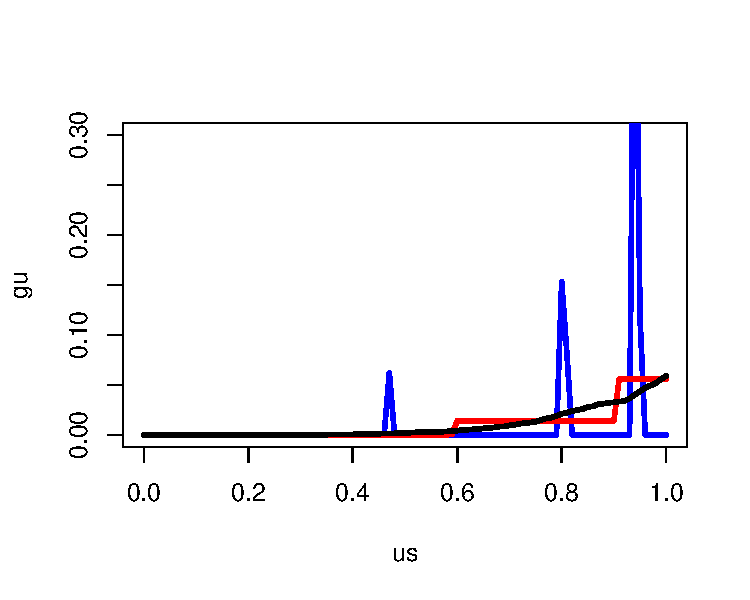
\includegraphics[scale = 0.5, clip=true, trim=0.2in 0.6in 0 0.7in]{../extrapolation/gu_est.pdf}} &
\multirow{5}{*}{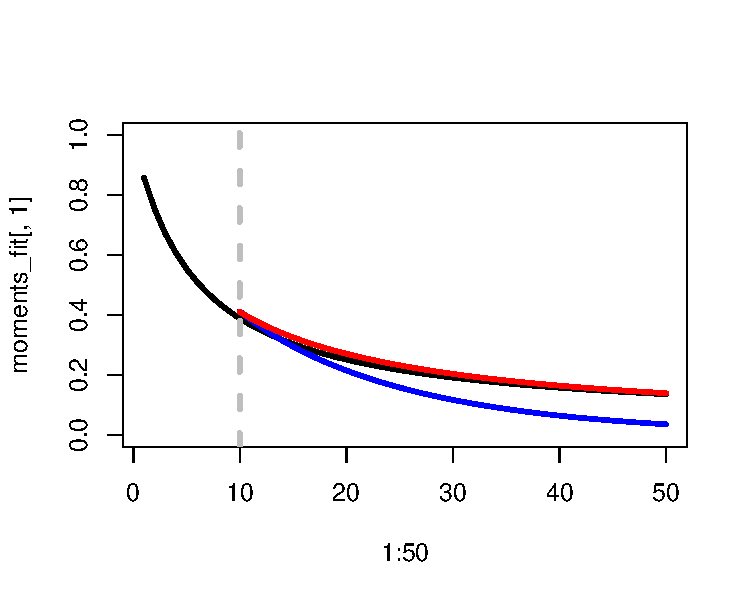
\includegraphics[scale = 0.5, clip=true, trim=0.2in 0.6in 0 0.7in]{../extrapolation/gu_est_moments.pdf}} & & \\
& & \crule[black]{0.2cm}{0.2cm} & Truth\\
& & & \\
& & \crule[blue]{0.2cm}{0.2cm} & MPLE \\
& & & \\
& & \crule[red]{0.2cm}{0.2cm} & CONS \\
& & & \\
& & & \\
& & & \\
$u$& $t$& & \\
\end{tabular}
\caption{Maximum pseudolikelihood (MPLE) versus constrained pseudolikelihood (CONS).
Adding constraints improves the estimation of the density $\eta(u)$, as well as moment estimation.}
\end{figure}

The (log) pseudolikelihood is defined as
\begin{equation}\label{eq:psuedo}
\ell(\eta) = \sum_{i=1}^k \sum_{j=1}^{m} \log\left(\int u^{V_{i, j}} (1-u)^{k - V_{i, j}} \eta(u) du\right),
\end{equation}
and a maximum pseudolikelihood estimator (MPLE) is defined as any
density $\hat{\eta}$ such that
\[
\ell(\hat{\eta}_{MPLE}) = \sup_{\eta} \ell(\eta).
\]
The motivation for $\hat{\eta}_{MPLE}$ is that it consistently
estimates $\eta$ in the limit where $k \to \infty$.
However, in finite samples, $\hat{\eta}_{MPLE}$ is not uniquely defined,
and if we define the plug-in estimator
\[
\hat{p}_t^{MPLE} = \int u^{t-1} \hat{\eta}_{MPLE}(u) du,
\]
$\hat{p}_t^{MPLE}$ can vary over a large range, depending on which $\hat{\eta} \in \argmax_{\eta} \ell_t(\eta)$
is selected.
These shortcomings motivate the adoption of additional constraints on the estimator $\hat{\eta}$.

Theorem 3.4. motivates the \emph{monotonicity constraint} that $\frac{d\hat{\eta}}{du} > 0$.
A second constraint is to restrict the $k$-th moment of $\hat{\eta}$ to match the unbiased estimate.
The addition of these constraints yields the constrained PMLE
$\hat{\eta}_{CON}$, which is obtained by solving
\[
\text{maximize }\ell(\eta) \text{ subject to }\int u^{k-1} \eta(u) du = \hat{p}_k^{UN}\text{ and }\frac{d\hat{\eta}}{du} > 0.
\]
By discretizing $\eta$, all of the above maximization problems can be solved using a general-purpose convex solver\footnote{
We found that the disciplined convex programming language CVX, using the ECOS second-order cone programming solver,
succeeds in optimizing the problems where the dimension of the discretized $\eta$ is as large as 10,000 [10, 11].}.
While the added constraints do not guarantee a unique solution,
they improve estimation of $\eta$ and thus improve moment estimation (Figure 1.)


\subsection{High-dimensional asymptotics}

Under a number of conditions on the distribution $\mathbb{F}$, including (but not limited to) having a large dimension $p$,
Anon [4] relate the accuracy $p_t$ of the Bayes classifier to the mutual information between the label $z$ and
the response $y$:
\[
p_t = \bar{\pi}_t(\sqrt{2I(Z; Y)}).
\]
where
\[
\bar{\pi}_k(c) = \int_{\mathbb{R}} \phi(z - c)  \Phi(z)^{k-1} dz.
\]
While our goal is not to estimate the mutual information, we note that the results of Anon 2016
imply a relationship between $p_k$ and $p_K$ for the Bayes accuracy under the high-dimensional regime:
\[
p_K = \bar{\pi}_K\left(\bar{\pi}_k^{-1}(p_k)\right).
\]
Therefore, under the high-dimensional conditions of [4] and assuming that the classifier approximates
the Bayes classifier, we naturally obtain the following estimator
\[
\hat{p}_t^{HD} = \bar{\pi}_K\left(\bar{\pi}_k^{-1}(\hat{p}_k^{UN})\right).
\]

\section{Results}

We applied the methods described in Section 4 on a simulated gaussian mixture (Figure 2)
and on a Telugu character classification task [12] (Table 1.)

For the simulated gaussian mixture, we vary the size of the initial subset from $k=3$ classes to $k=K=50$ classes,
and extrapolate the performance for gaussian mixture model, multinomial logistic, and one-layer neural network (with 10 sigmoidal units.)
Figure 3 shows how the predicted $K$-class accuracy changes as $k$ is varied.
We see that the predicted accuracy curves for QDA and Logistic have similar behavior,
even though QDA is generative and multinomial logistic is not.  All three methods perform better on QDA and logistic classifiers
than on the neural network: in fact, for the neural network, the test accuracy of the initial set, $\text{acc}^{(k)}$,
becomes a better estimator of $\text{acc}^{(K)}$ than the three proposed methods for most of the curve.
We also see that the exponential extrapolation method, $\hat{p}^{EXP}$,
is more variable than constrained pseudolikelihood $\hat{p}^{CONS}$ and high-dimensional estimator $\hat{p}^{HD}$.
Additional simulation results can be found in the supplement.

In the character classification task, we predict the 400-class accuracy of naive Bayes, multinomial
logistic regression, SVM [6], $\epsilon$-nearest neighbors\footnote{$k$-nearest neighbors with $k = \epsilon n$ for fixed $\epsilon > 0$}, and deep neural networks\footnote{The network architecture is as follows: 
{\tt 48x48-4C3-MP2-6C3-8C3-MP2-32C3-50C3-MP2-200C3-SM.}
48x48 binary input image, $m$C3 is a 3x3 convolutional layer with $m$ output maps, MP2 is a 2x2 max-pooling layer, and SM is a softmax output layer on 20 or 400 classes.} using 20-class data with 103 training examples per class (Table 1).
Taking the test accuracy on 400 classes (using 50 test examples per class) as a proxy for $\text{acc}^{(400)}$,
we compare the performance of the three extrapolation methods; as a benchmark,
also consider using the test accuracy on 20 classes as an estimate.
The exponential extrapolation method performs well only for the deep neural network.  Meanwhile, constrained PMLE achieves accurate extrapolation for two out of four classifiers: logistic and SVM
but failed to converge for the the deep neural network (due to the high test accuracy).
The high-dimensional estimator $\hat{p}^{HD}$  performs well on the multinomial logistic, SVM, and deep neural network classifiers.  All three methods beat the benchmark (taking the test accuracy at 20) for the first four classifiers;
however, the benchmark is the best estimator for the deep neural network,
similarly to what we observe in the simulation (albeit with a shallow network rather than a deep network.)

\begin{figure}
\centering
\begin{tabular}{cccrl}
QDA & Logistic & Neural Net & \\
\multirow{5}{*}{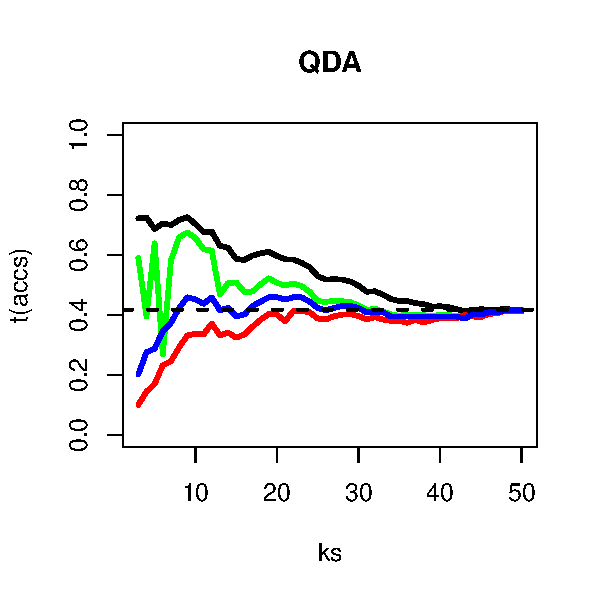
\includegraphics[scale = 0.5, clip=true, trim=0.2in 0.6in 0.2in 0.7in]{../extrapolation/sim_qda.pdf}} &
\multirow{5}{*}{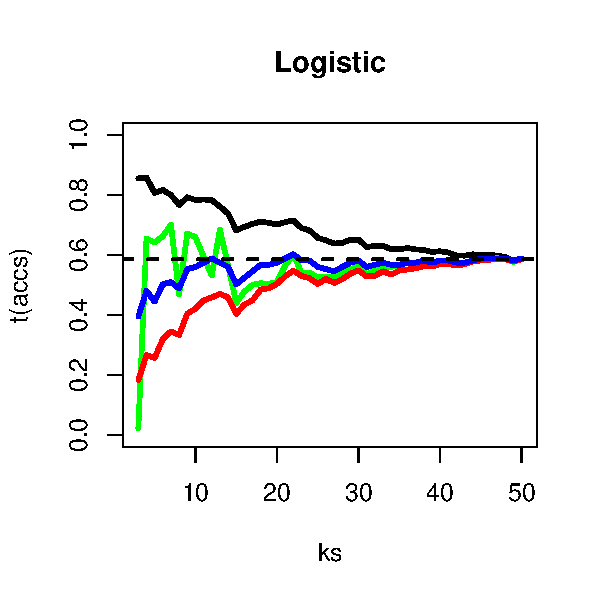
\includegraphics[scale = 0.5, clip=true, trim=0.75in 0.6in 0.2in 0.7in]{../extrapolation/sim_glmnet.pdf}} & 
\multirow{5}{*}{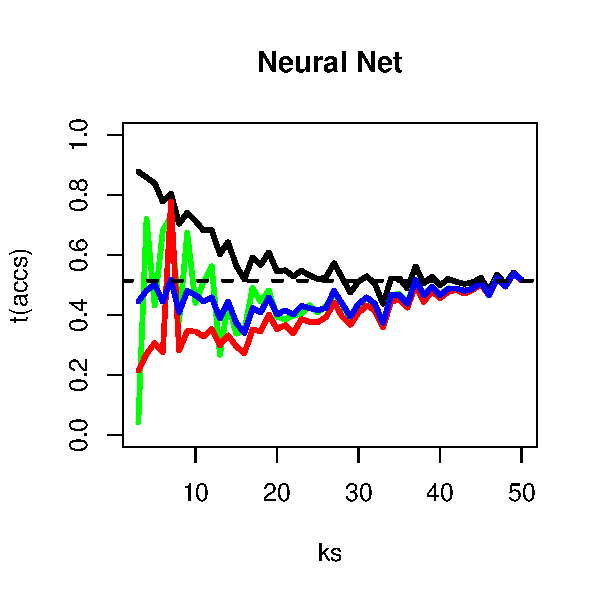
\includegraphics[scale = 0.5, clip=true, trim=0.75in 0.6in 0.2in 0.7in]{../extrapolation/sim_nnet.pdf}} & 
& \\
&& & &\\
&& &  \crule[black]{0.2cm}{0.2cm} & $\text{acc}^{(k)}$ \\
&& & \crule[green]{0.2cm}{0.2cm} & $\hat{p}^{EXP}$ \\
&& & \crule[red]{0.2cm}{0.2cm} & $\hat{p}^{CONS}$ \\
&& & \crule[blue]{0.2cm}{0.2cm} & $\hat{p}^{HD}$ \\
&& & & \\
&& & & \\
&& & & \\
$k$ &$k$& $k$& & \\
\end{tabular}
\caption{Predictions for $\text{acc}^{(50)}$ as $k$, the size of the subset, is varied.  Our methods work better for QDA and Logistic than Neural Net; overall, $\hat{p}^{EXP}$ has higher variability than $\hat{p}^{CONS}$ and $\hat{p}^{HD}$.}
\end{figure}

\begin{table}
\centering
\begin{tabular}{|c||c|c|c|c|c|}\hline
Classifier & Test $\text{acc}^{(20)}$ & Test $\text{acc}^{(400)}$ & $\hat{p}^{EXP}_{400}$ & $\hat{p}^{CONS}_{400}$ & $\hat{p}^{HD}_{400}$\\ \hline
Naive Bayes & 0.947 & 0.601 & 0.884 & \textbf{0.659} & 0.769 \\ \hline
Logistic & 0.922 & 0.711 & 0.844 & \textbf{0.682} & 0.686 \\ \hline
SVM & 0.860 & 0.545 & 0.737 & 0.473 & \textbf{0.546} \\ \hline
$\epsilon$-NN & 0.964 & 0.591 & 0.895 & \textbf{0.395} & 0.839\\ \hline
Deep neural net & \textbf{0.995} & 0.986 & 0.973 & (*) & 0.957\\ \hline
\end{tabular}
\caption{Performance extrapolation: predicting the accuracy on 400 classes using data from 20 classes on a Telugu character dataset. (*) indicates failure to converge.
$\epsilon = 0.002$ for $\epsilon$-nearest neighbors.}
\end{table}

\section{Discussion}

Empirical results indicate that our methods generalize beyond generative classifiers.
A possible explanation is that since the Bayes classifier is generative,
any classifier which approximates the Bayes classifier is also `approximately generative.'
However, an important caveat is that the classifier must already attain close to the Bayes accuracy
on the smaller subset of classes.  If the classifier is initially far from the Bayes classifier,
and then becomes more accurate as more classes are added, our theory could underestimate the
accuracy on the larger subset.  This is a non-issue for generative classifiers when the training data per class is fixed,
since a generative classifier approximates the Bayes rule if and only if the single-class classification function approximates the
Bayes optimal single-class classification function.  On the other hand, for classifiers with built-in \emph{model selection}
or \emph{representation learning}, it is expected that the classification functions become more accurate,
in the sense that they better approximate a monotonic function of the Bayes classification functions,
as data from more classes is added.

Our results are still too inconclusive for us to recommend the use of any of these estimators in practice.
Theoretically, it still remains to derive confidence bounds for the generative case;
practically, additional experiments are needed to establish the reliability of these estimators
in specific applications.  There also remains plenty of room for new and improved estimators in this area:
for instance, fixing the instability of the constrained pseudolikelihood estimator when the test accuracy is high.

%\begin{figure}
%\centering
%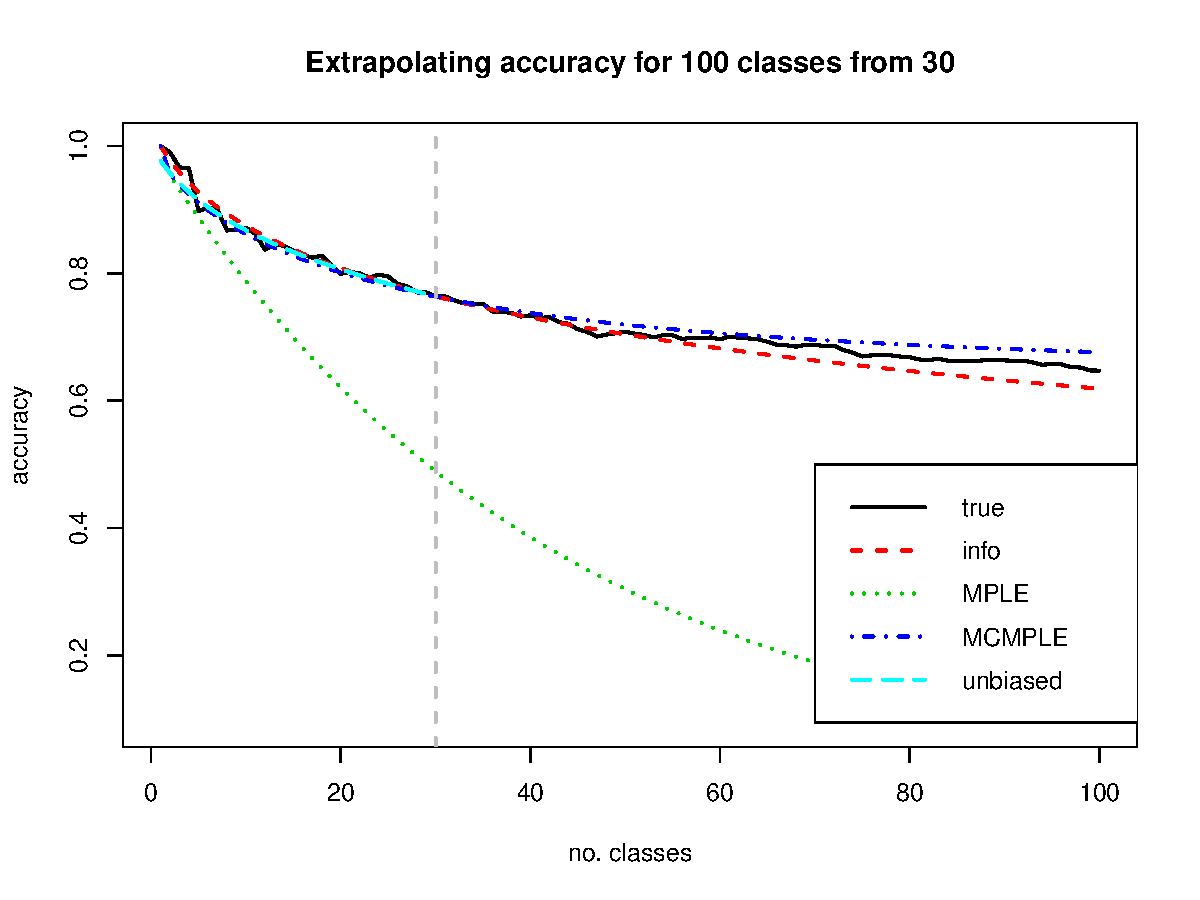
\includegraphics[scale = 0.6]{cifar_example.pdf}
%\caption{Extrapolation classification performance for CIFAR data.  (This simulation needs to be fixed later.)
%PMLE: maximum psuedolikelihood. MCPMLE: Moment-constrained max psuedolikelihood.  Info: Zheng and Benjamini's info-%theoretic method.
%Unbiased: U-statistic (cannot be used to extrapolate.) }
%\end{figure}


%\subsubsection*{Acknowledgments}

%We thank John Duchi, Steve Mussmann, Qingyun Sun, Jonathan Taylor, Trevor Hastie, Robert Tibshirani for useful discussion.  CZ is supported by an NSF graduate research fellowship.

\section*{Appendix}

\noindent\textbf{Theorem 3.1.} \emph{
Let $\mathcal{Q}$ be a single-distribution classification function, and let $\mathbb{F}$, $\hat{\mathbb{F}}(F)$ be a distribution on $\mathcal{P}(\mathcal{Y}).$
Further assume that
$\hat{\mathbb{F}}$ and $\mathcal{Q}$ jointly satisfy the
\emph{tie-breaking} property:
\begin{equation}\label{eq:tie}
\Pr[\mathcal{Q}(\hat{F}, y) = \mathcal{Q}(\hat{F}', y)] = 0
\end{equation}
for all $y \in \mathcal{Y}$, where $\hat{F}, \hat{F}' \stackrel{iid}{\sim} \hat{\mathbb{F}}$.
Let $U$ be defined as the random variable
$U = u(\hat{F}, Y)$
for $F \sim \mathbb{F}$, $Y \sim F$, and $\hat{F} \sim \hat{\mathbb{F}}(F)$ with $Y \perp \hat{F}$.
Then \[p_k = \E[U^{k-1}],\]
where $p_k$ is the expected accuracy as defined by \eqref{eq:pt}.
}


\noindent\textbf{Proof.}  
Write $q^{(i)}(y) = \mathcal{Q}(\hat{F}_i, y)$.
By using conditioning and
conditional independence, $p_k$ can be written
\begin{align*}
p_k &= \E\left[ \frac{1}{k}\sum_{i=1}^k  \Pr_{F_i}[q^{(i)}(Y) > \max_{j\neq i} q^{(j)}(Y)] \right]
\\&= \E\left[ \Pr_{F_1}[q^{(1)}(Y) > \max_{j\neq 1} q^{(j)}(Y)] \right]
\\&= \E_{F_1}[\Pr[q^{(1)}(Y) > \max_{j\neq 1} q^{(j)}(Y)|\hat{F}_1, Y]]
\\&= \E_{F_1}[\Pr[\cap_{j > 1} q^{(1)}(Y) > q^{(j)}(Y)|\hat{F}_1, Y]]
\\&= \E_{F_1}[\prod_{j > 1}\Pr[q^{(1)}(Y) > q^{(j)}(Y)|\hat{F}_1, Y]]
\\&= \E_{F_1}[\Pr[q^{(1)}(Y) > q^{(2)}(Y)|\hat{F}_1, Y]^{k-1}]
\\&= \E_{F_1}[u(\hat{F}_1, Y)^{k-1}] = \E[U^{k-1}].
\end{align*}
$\Box$


\section*{References}

\small

[1] Kay, K. N., Naselaris, T., Prenger, R. J., \& Gallant, J. L. (2008). ``Identifying natural images from human brain activity.'' 
\emph{Nature}, 452(March), 352-355.

[2] Deng, J., Berg, A. C., Li, K., \& Fei-Fei, L. (2010). ``What does classifying more than 10,000 image categories tell us?'' \emph{Lecture Notes in Computer Science}, 6315 LNCS(PART 5), 71-84. 

[3] Garfield, S., Stefan W., \& Devlin, S. (2005). ``Spoken language classification using hybrid classifier combination." 
\emph{International Journal of Hybrid Intelligent Systems} 2.1: 13-33.

[4] Anonymous, A. (2016). ``Estimating mutual information in high dimensions via classification error.''  Submitted to 
\emph{NIPS 2016.}

[5] Tewari, A., \& Bartlett, P. L. (2007). ``On the Consistency of Multiclass Classification Methods.''
\emph{Journal of Machine Learning Research}, 8, 1007-1025.

[6] Hastie, T., Tibshirani, R., \& Friedman, J., (2008). \emph{The elements
of statistical learning.} Vol. 1. Springer, Berlin: Springer series in
statistics.

[7] Arnold, Barry C., \& Strauss, D.  (1991). ``Pseudolikelihood estimation: some examples." \emph{Sankhya: The Indian Journal of Statistics, Series B}: 233-243.

[8] Cox, D.R., \& Hinkley, D.V. (1974). \emph{Theoretical statistics.} Chapman and Hall. ISBN 0-412-12420-3

[9] Lawson, C. L., \& Hanson, R. J. (1974). \emph{Solving least squares problems.} Vol. 161. Englewood Cliffs, NJ: Prentice-hall.

[10] Hong, J., Mohan, K. \& Zeng, D. (2014). ``CVX. jl: A Convex Modeling Environment in Julia."

[11] Domahidi, A., Chu, E., \& Boyd, S. (2013). "ECOS: An SOCP solver for embedded systems." \emph{Control Conference (ECC), 2013 European. IEEE.}

[12] Achanta, R., \& Hastie, T. (2015) "Telugu OCR Framework using Deep Learning." arXiv preprint arXiv:1509.05962 .

\end{document}


